% iaus2esa.tex -- sample pages for Proceedings IAU Symposium document class
% v1.04,  Copyright (2004) International Astronomical Union

\NeedsTeXFormat{LaTeX2e}

\documentclass{iau}
% Include figures (EPS only), using e.g.:
\usepackage{graphicx} 


%% -- Title ------------------------------------
\title[Multiwavelngth Astronomy ~~PSR J0737$-$3039] %% short title %%
{Using the Universe as a Physics Laboratory: A Multiwavelength Review of PSR J0737$-$3039} %% full title %%

%% -- Authors ----------------------------------
\author[Umang Mishra]  %% short author list %%
{Umang Mishra $^1$}
% \thanks{Present address: ...},
%% \and Author Two$^2$}

\affiliation{New York University Abu Dhabi\\ email: {\tt um339@nyu.edu}} 
%%\\[\affilskip]
%%$^2$A, \\ B \\email: {\tt c@d.com}}

%% -- Header (pre-filled, do not edit) -----------------
%\pubyear{2012}
%\volume{1}  %% insert here IAU Symposium No.
% \pagerange{1--9}
% \date{?? and in revised form ??}
% \setcounter{page}{1}
%\jname{\mbox{Multi-Wavelength Astronomy: Final Reports of Sources Studied in Depth}}
%\editors{M. S. E. Roberts , ed.} 
\begin{document}

\maketitle

%% -- Abstract ----------------------------------
\begin{abstract}

This paper is a multi-wavelength review of the double pulsar binary PSR J0737$-$3039. 
(more will be added once the entire paper is finished).

%% add here a maximum of 10 keywords, to be taken form the file <Keywords.txt>
\keywords{PSR J0737$-$3039,Double Pulsar Binary, General Relativity}
\end{abstract}

% add below any authors, subjects and objects for indexing 
%   add more lines if necessary
%   but leave all lines commented out
%\index[author]{LastName1, Initials|textbf}
%\index[author]{LastName2, Initials|textbf}
%\index[subject]{Keyword1}
%\index[subject]{Keyword2}
%\index[object]{Object1}
%\index[object]{Object2}


\firstsection % if your document starts with a section,
              % remove some space above using this command.
\section{Introduction}
The double pulsar binary system J0737$-$3039 was discovered in 2004 using the Parkes 64-m radio telescope in New South Wales, Australia by \cite{b03}. Right from its discovery, the pulsar binary was anticipated to be crucial towards better understanding of  Post Newtonian formalism and gravitational waves. J0737$-$3039A is a millisecond pulsar with 22.7ms period, and its counterpart is a young unrecycled pulsar with a period of 2.77 s as summarized by \cite{lyn06} . While initially the system was only observed in the radio wavelengths for testing general relativity, observations were also performed using XMM Newton in soft X-ray. Some observations in gamma ray have also been performed. (More info on X-Ray and gamma later)

\section{Radio Observations}

\subsection{The Discovery and the Parameters}
Although the first observation was made by the Parkes 64-m at 1390Hz, better precision was obtained after interferometric observations were made using the Australia Telescope Compact Array(ATCA). The pulsar A of the system was found to be in a 2.4 hour eccentric orbit with eccentricity of 0.088 by \cite{b03}. The ATCA measurements helped further measurement of parameters, giving a period of 22.699 ms for pulsar A. The period of pulsar B was found to be 2.8s by \cite{lyn04}.
 
The periastron advance($\dot\omega$) value was measured to be 16.88yr$^{-1}$ by the ATCA observations. This was the highest value of $\dot\omega$ and was used to predict the masses of the pulsars in the system.\cite{lyn04} also measured other post Keplerian parameters, and found that the predictions of masses were accurate. The system was thus established as a highly relativistic double pulsar binary system ideal for testing relativistic gravity.

\subsection{The Double Neutron System(DNS) as a Testing Ground for General Relativity}

\begin{figure}[h!]
	\begin{center}
		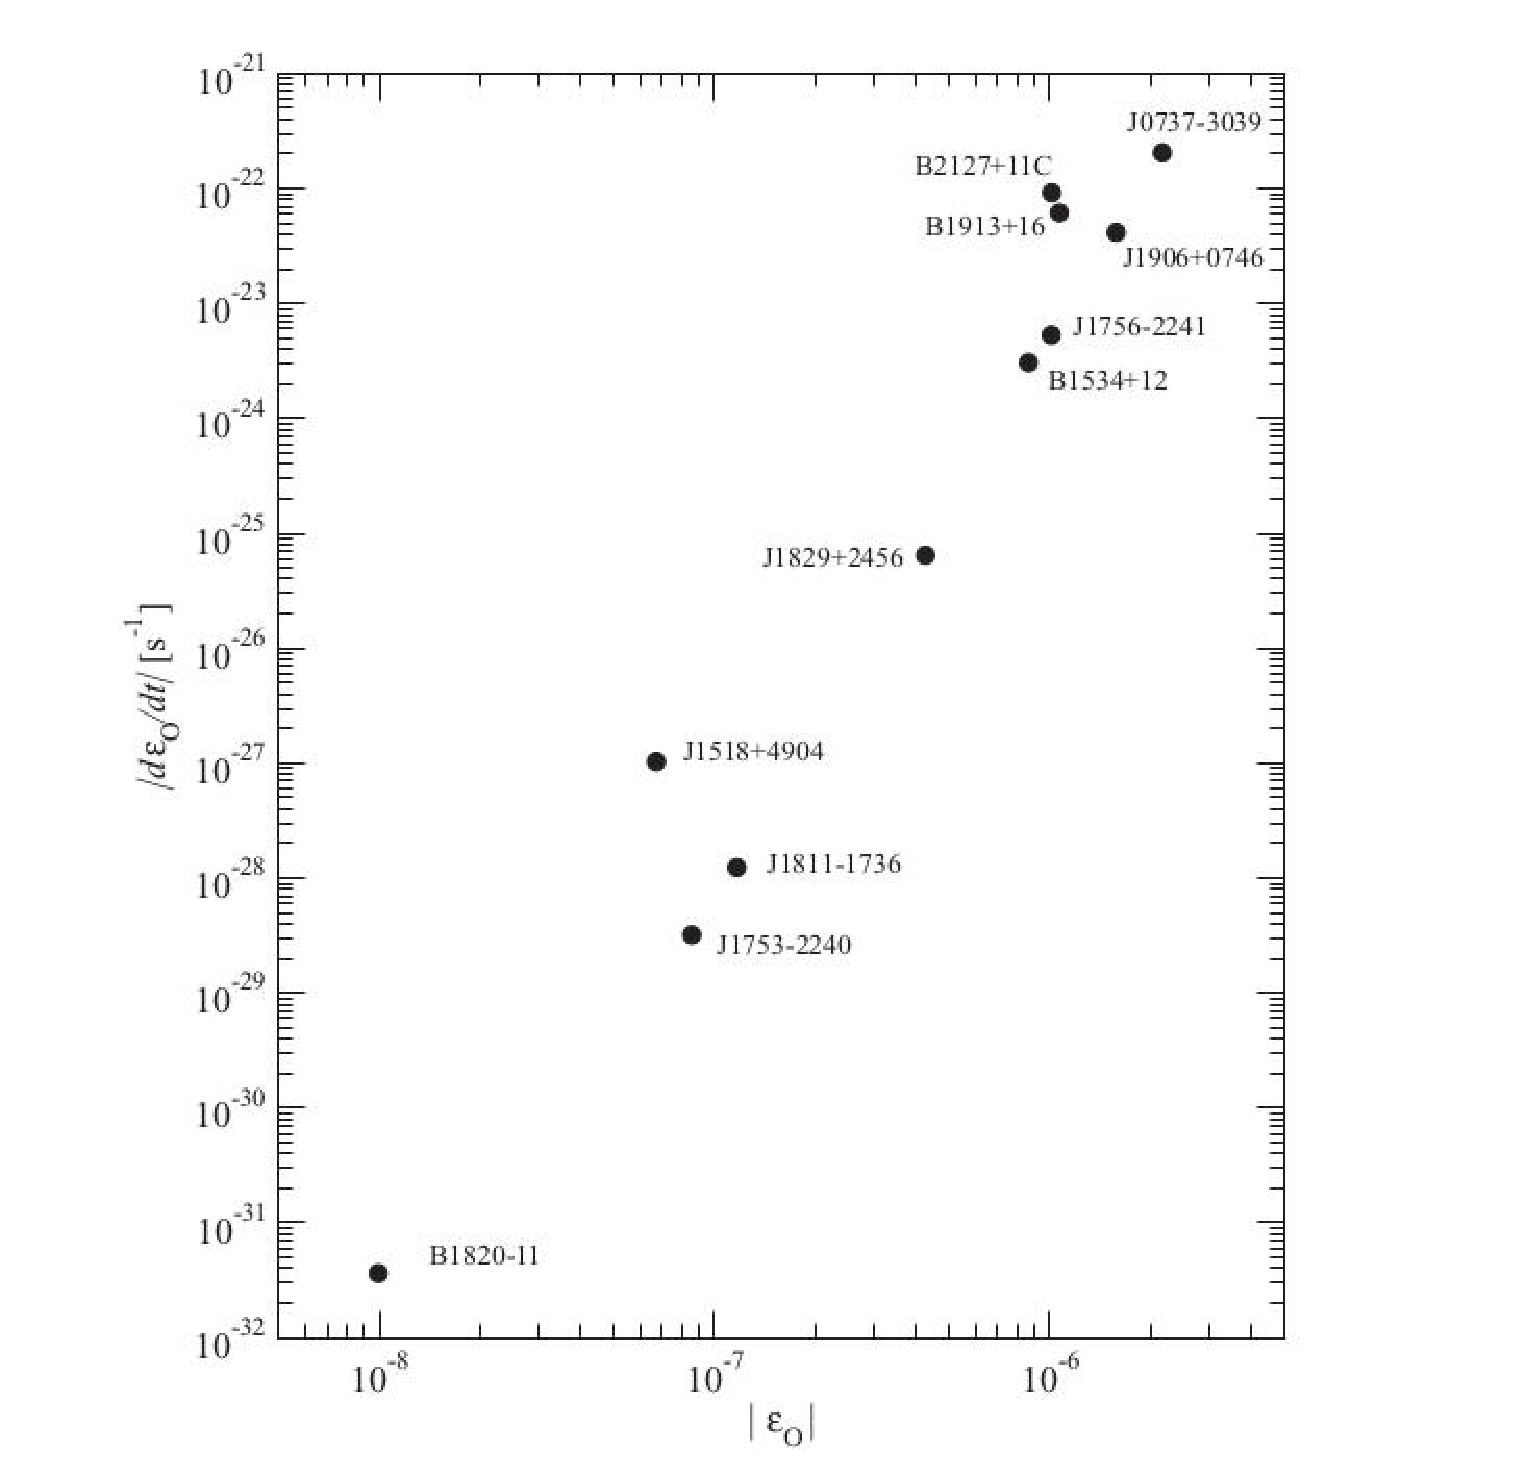
\includegraphics[width=3.4in]{fig1.eps} 
		\caption{Orbital energy-energy loss diagrams for known and likely double neutron binaries. $\epsilon_o$ is a direct measure for the strength of post-Newtonian effects in orbital dynamics. It can thus clearly be seen that J0737-3039 (top right) is the most suitable candidate for studying relativistic gravity. Image taken from \cite{kwex09} }
		\label{fig1}
	\end{center}
\end{figure}

Usually, five Keplerian Parameters are sufficient to describe binary systems. These are: P$_{orb}$, e, $\omega$, a$sin i$, and T$_o$. In case of strong gravitational interactions, such as in the case of a double neutron system, six additional parameters called the post-Keplerian parameters are required to fully describe the system due to relativistic effects that come into play. These are : $\dot\omega$, $\gamma$, $r$, $s$,dP$_b$/dt, and $\Omega_{SO}$. Since gravity is the only way stars in DNS interact, it makes them ideal candidates for studying relativistic gravity theories using these post-Keplerian parameters.

As shown in figure 1, PSR J0737-3039 is the most suitable system for studying relativistic gravity.  Each of the post-Keplerian(PK) parameters is related to the masses of the pulsars in the system in a unique way.With a system as J0737-3039, a ratio of stellar masses can be obtained from observations and plotted as a straight line according to the equation: \[\frac{a_B sini}{a_A sini}=\frac{m_A}{m_b}\]
An intersection between this line and the curves plotted for each PK on a mass-mass plot could be used as a verification test for general relativity. 

In the case of PSR J0737-3039, all five PK parameters can be measured for pulsar A. Since the equations for $\dot\omega$, $s$, and dP$_b$/dt for general relativity are symmetric in masses, they will be the same for both pulsar A and pulsar B. Studies of eclipses of A allow for measurement of $\Omega_{SO}$ for B. The mass-mass plot for these parameters, can be seen in figure 2. While all the experimental values agree within the error boundaries with the theoretical predictions, the best match is with Shapiro delay(with uncertainty of 0.05%).
 
\subsection{Insight into Pulsar Magnetospheres}

At conjunction, the line of sight of the two pulsars is within 0.15 ls of each other. As they further advance in their orbits, A is completely eclipsed by B and the line of sight of A sweeps through the magnetosphere of B. \cite{lyn04} suggested that studying the changes in radio transmission during this process that lead to understanding the physical conditions of B's magnetosphere, giving a better understanding of the plasma density and  magnetic field structure. 

\subsection{The Confirmation of DNS evolutionary Sequence}







% CUP work flow only accepts EPS -- not PDF, JPG, etc.
\begin{figure}[b]
\begin{center}
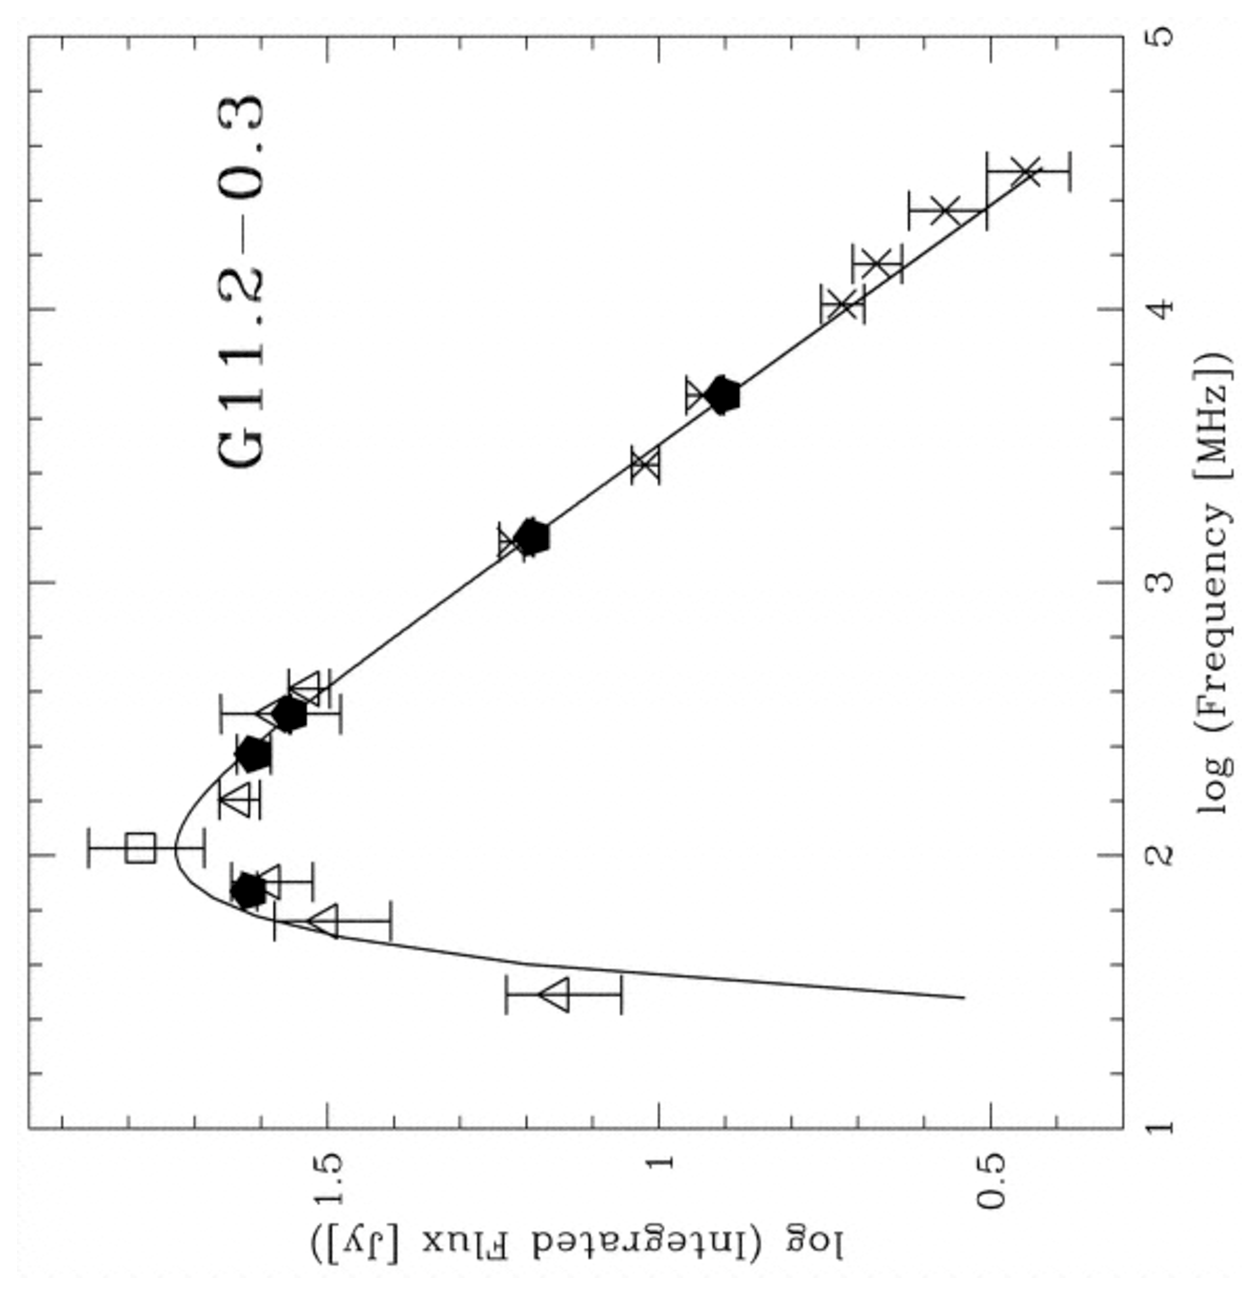
\includegraphics[width=3.4in,angle=270]{fig2.eps} 
\caption{Radio continuum spectrum for the shell of SNR G11.2-0.3. To account for the PWN flux, 1 Jy has been subtracted from the 
integrated flux measurements for data with $\nu > 200$ MHz, assuming that $\alpha_{PWN} \sim 0.0$ (from Brogan et al. 2004).}
\label{fig2}
\end{center}
\end{figure}


\begin{thebibliography}{}

\bibitem[Burgay et al. (2003)]{b03} Burgay, M., N. D’Amico, A. Possenti, R. N. Manchester, A. G. Lyne, B. C. Joshi, M. A. McLaughlin, et al. 2003. Nature 426 (6966): 531–33. https://doi.org/10.1038/nature02124.

\bibitem[Lyne (2006)]{lyn06} Lyne, A.G., 2006. Chinese Journal of Astronomy and Astrophysics Supplement 6, 162.

\bibitem[Lyne et al. (2004)]{lyn04} Lyne, A.G., Burgay, M., Kramer, M., Possenti, A., Manchester, R.N., Camilo, F., McLaughlin, M.A., Lorimer, D.R., D’Amico, N., Joshi, B.C., Reynolds, J., Freire, P.C.C., 2004. Science 303, 1153–1157.

\bibitem[Kramer and Wex (2009)]{kwex09} Kramer, M., Wex, N., 2009. Class. Quantum Grav. 26, 073001.

\end{thebibliography}


\end{document}
